\documentclass[9pt,twocolumn,twoside]{styles/osajnl}
\usepackage{fancyvrb}
\journal{i524} 

\title{CDAP Cask Data Application Platform}

\author[1,*, +]{Avadhoot Agasti}

\affil[1]{School of Informatics and Computing, Bloomington, IN 47408, U.S.A.}

\affil[*]{Corresponding authors: aagasti@indiana.edu}

\affil[+]{HID - SL-IO-3000}

\dates{project-000, \today}

\ociscodes{CDAP, Hadoop, Name Node, Edge Node, Yarn, Apache Sqoop, Apache
Flume, Apache Flink, Apache Atlas, HDFS, Apache Kafka, Apache Spark,
MapReduce, HBase}

% replace this with your url in github/gitlab
\doi{\url{https://github.com/avadhoot-agasti/sp17-i524/tree/master/paper1/S17-IO-3000/report.pdf}}


\begin{abstract}
CDAP provides application development platform on top of Apache Hadoop. CDAP
services enable users to automate the task of building, executing and
managing data pipelines. The CDAP studio allows users to drag-and-drop data
sources, transformation tasks, and data sinks. User can chain these tasks to
create data pipelines. Furthermore, CDAP provides abstraction of logical data
pipeline over execution environment. Using CDAP, user can execute a data
pipeline either using MapReduce or Apache Spark depending on the capability
of underlying Hadoop cluster.
\newline
\end{abstract}

\setboolean{displaycopyright}{true}

\begin{document}

\maketitle

\section{Introduction}

CDAP stands for Cask Data Application Platform \cite{www-cask-io}. CDAP is an
application development platform that can help developers build, deploy and
 monitor applications on Apache Hadoop. In a CDAP application, a
 developer can ingest a dataset, store and manage it on Hadoop, perform
 data analysis, and develop web services to expose the original and
 transformed dataset(s). He can also schedule and monitor the execution of
 the application. CDAP enables the developers to use single platform to
 develop the end-to-end application on Apache Hadoop.

This technology paper is structured as follows:
\begin{itemize}
\item Section 2 explains commonly used application architecture on top of
Apache Hadoop without using CDAP. It then explains the application
architecture using CDAP to ephasize the use of CDAP.
\item Section 3 explains important CDAP concepts.
\item Section 4 and Section 5 explain the CDAP deployment options and
infrastructure requirements.
\item Section 6 explains the representative use cases.
\item Section 7 and 8 provide useful information about CDAP like licensing
and educational material.
\item Finally, in Section 9 and 10, we conclude by explaining the other similar
platforms and their high level comparison with CDAP
\end{itemize}

\section{CDAP: Unified Application Development Platform}
CDAP provides a unified application development platform on top of Apache
Hadoop. In below sections, we explain a commonly used application
architecture on top of Apache Hadoop. Then we explain the CDAP application
architecture using which different components of the application architecture
 are unified in CDAP platform.

\subsection{Application Architecture on Hadoop without CDAP}
Figure 1 \cite{www-hdp-dataplatform} shows a commonly used application
architecture on Hadoop (without CDAP).


\begin{figure}[htbp]
\centering
\fbox{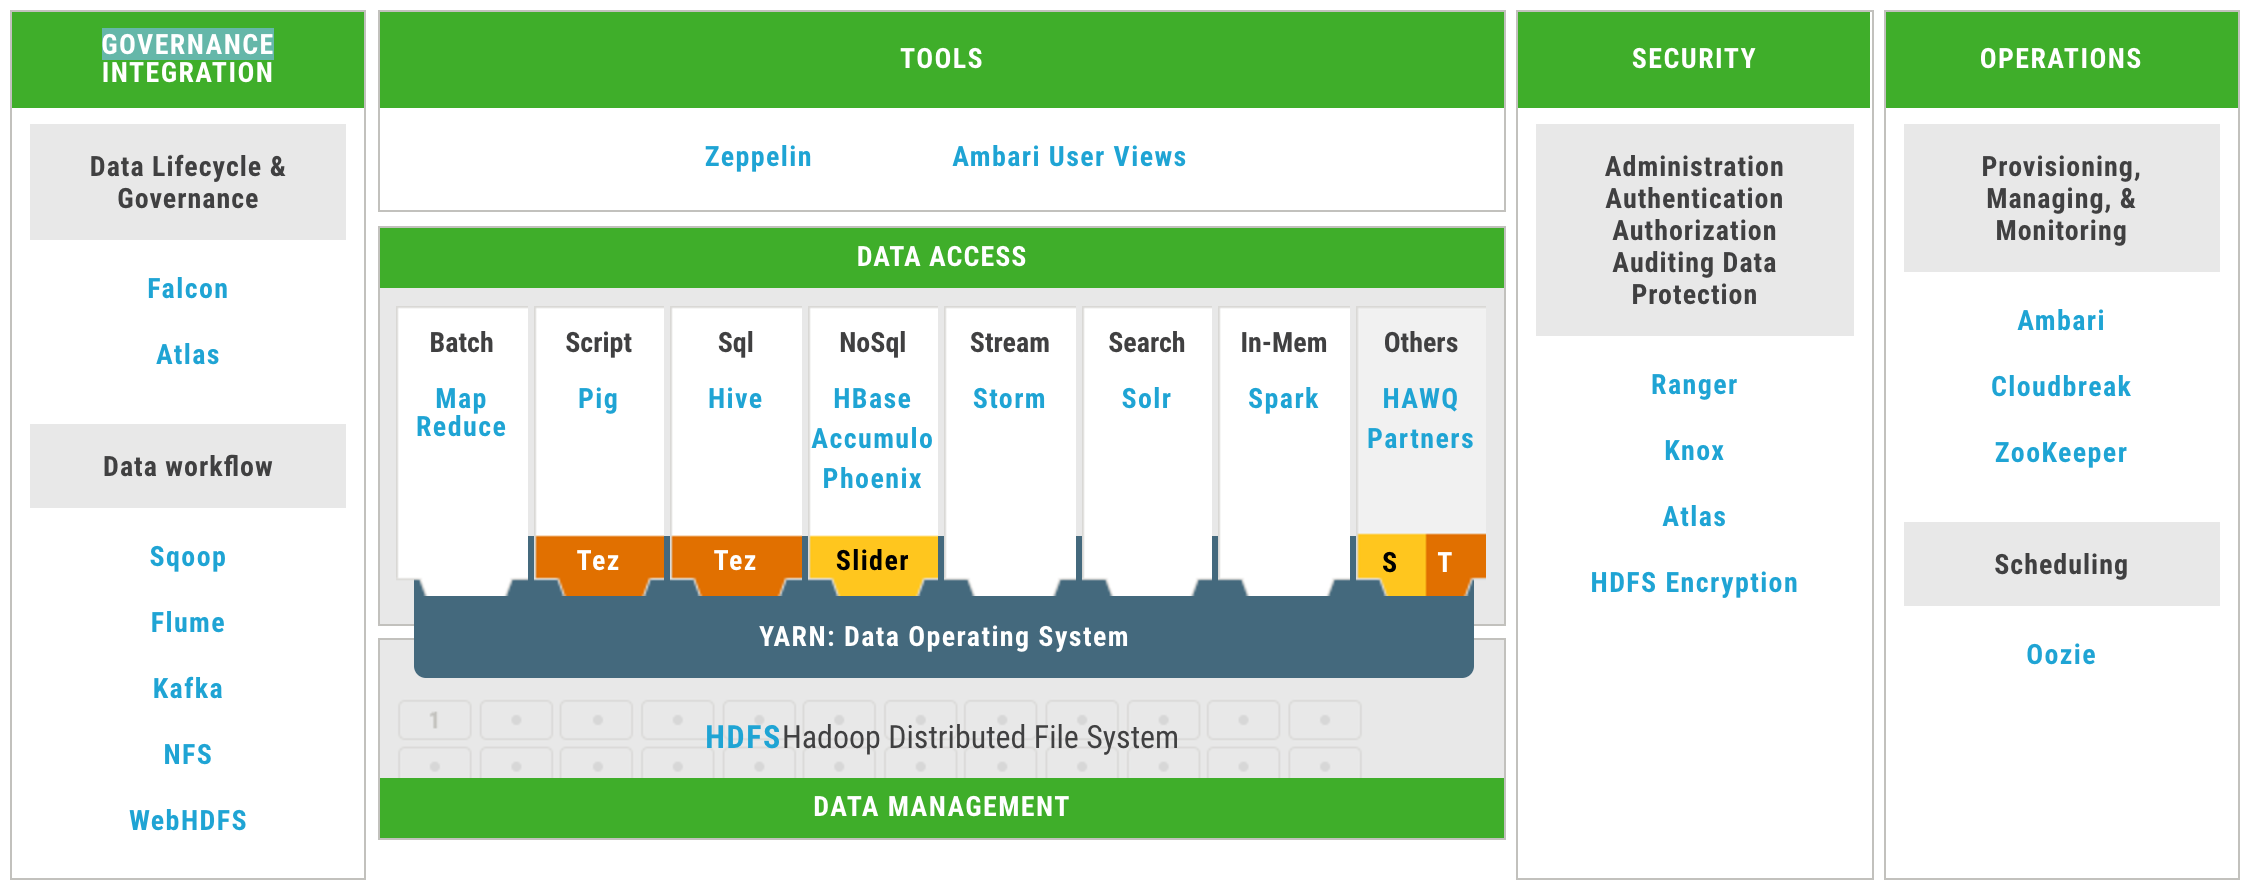
\includegraphics[width=\linewidth]{images/hdp-application-arch.png}}
\caption{Application Architecture on Hadoop.}
\label{fig:hadoop-arch}
\end{figure}

There are following layers/components as depicted in the architecture diagram
\cite{www-hdp-dataplatform}.

\begin{itemize}
\item Data Governance and Integration: This layer is responsible for ingesting
the data from data source into Hadoop. Data Ingestion tools like Apache
Sqoop, Apache Flume and Apache Kafka are used for Data Ingestion while Apache
Falcon and Apache Atlas are used for Data Lifecycle management.
\item Data Storage: The data is stored in HDFS.
\item Data Processing and Access: The data is transformed and aggregated in
Data Processing layer. The processing can involve various steps like cleansing,
joining, aggregation and running machine learning algorithms. Many different
tools and technologies are used to perform data processing operations.
PIG, Hive, Spark are open source scripting technologies which can perform
Data Processing tasks.
\item Tools: Tools like Apache Zeppelin provide user interface to visualize
the data.
\item Security and Operations: The data pipeline built using above tools can
 be secured using tools such as Ranger, Knox, and Atlas. The scheduling of
 the data pipeline is orchestrated using Oozie.
\end{itemize}

This application architecture explains that an application built on top
 of Apache Hadoop involve multiple tools and technologies. Further it is
 tightly dependent on the underlying deployment architecture and tools
 availability. Using this mechanism, it is difficult to segregate the
 application business logic from infrastructure components.

\subsection{Application Architecture on Hadoop with CDAP}
Figure 2 \cite{www-cdap-architecture} explains how CDAP provides a common
application development platform. CDAP provides abstractions to ingest data,
store it in HDFS, process it using the application business logic, store the
results in HDFS and expose web service APIs on the result data. Developers need
 not use different tools to implement various layers. He can implement
  all the layers in CDAP platform. Further, he can use Java as a common coding
 language to implement all the coding tasks across all the layers.

\begin{figure}[htbp]
\centering
\fbox{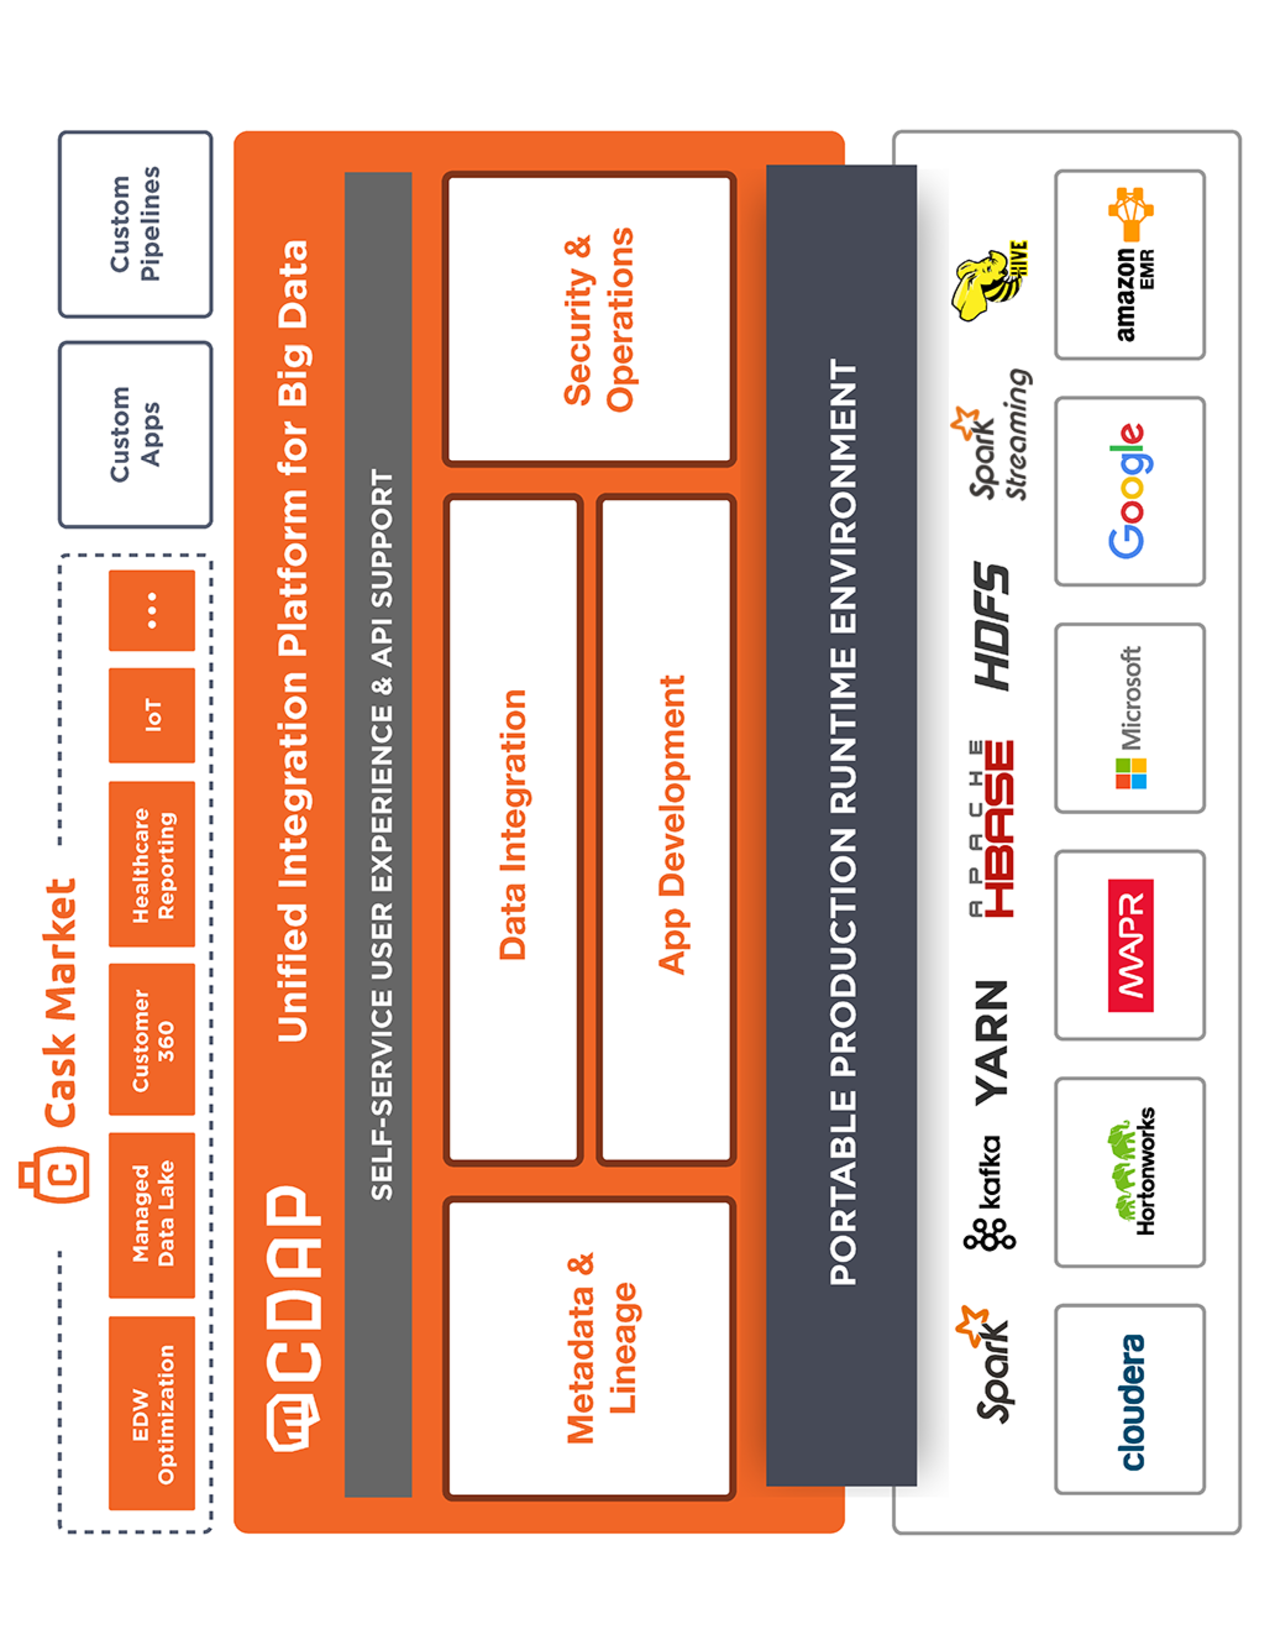
\includegraphics[width=\linewidth]{images/cdap-architecture.png}}
\caption{CDAP Application Architecture.}
\label{fig:CDAP Architecture}
\end{figure}

\section{Important CDAP Concepts}
CDAP revolves around below important concepts:
\begin{itemize}
\item CDAP Datasets provide logical abstraction over the data stored in
Hadoop. The data can be files in HDFS or tables in HBase. A dataset needs to
be first declared in the CDAP. Any dataset declared in CDAP can be used in
any CDAP applications or CDAP services.
\item CDAP Applications provide containers to implement application business
logic in open source processing frameworks like MapReduce, Spark and real
time flow. CDAP applications also provide standardize way to deploy and
manage the apps
\item CDAP Services provide services for application management, metadata
management, and streams management
\end{itemize}

\section{CDAP Deployment}
CDAP provides multiple deployment options. In standalone mode, it can be
downloaded as a zip file and deployed.
Alternatively it is available as a standalone virtual machine.
For deployment in cluster mode, CDAP provides options which are specific to
underlying Hadoop distribution as explained below:
\begin{itemize}
\item Cloudera Hadoop Distribution (CDH) - Cloudera Manager
\cite{www-cdh-manager} is tool to deploy CDH cluster. CDAP provides
CDAP-parcel \cite{www-cdap-cloudera-manager} which is plug in for
Cloudera Manager. Once you add CDAP-parcel to your Cloudera Manager, CDAP can
 be deployed using Cloudera Manager and all CDAP services can be monitored
 using Cloudera Manager.
\item Amazon EMR (Elastic Map Reduce) - EMR is Amazon's Hadoop distribution
for the Amazon Web Services cloud \cite{www-amazon-emr}.  EMR provides
'Create Cluster Wizard' to create EMR cluster. According the CDAP
documentation \cite{www-cdap-emr}, CDAP provides a bootstrap action which is
executed when the EMR cluster is created. Using this mechanism, CDAP platform
 can be deployed on EMR when the EMR cluster is created.
\item
CDAP can also be deployed on HortonWorks Hadoop Distribution, MapR Hadoop
Distribution and Apache Hadoop.
\end{itemize}



\section{CDAP Infrastructure Requirements}

CDAP is deployed on edge nodes of the Hadoop cluster. CDAP communicates with
Hadoop services like Yarn, HDFS and HBase. Hence CDAP needs to be installed
in same network as that of Hadoop. However, none of the CDAP components are
required to be installed on Hadoop Namenode or Hadoop datanodes. CDAP
documentation \cite{www-cdap-deployment} provide the CDAP deployment
architecture.

\section{Representative Use Cases}

CASK \cite{www-cask-io} is the company which provides commercial distribution
for CDAP. CASK has developed several applications using CDAP.
Some of the applications developed using CDAP are explained below
\begin{itemize}
\item CASK Hydrator \cite{www-cask-hydrator} is interactive application for
building, running and managing data pipelines for enterprise data lake.
CASK Hydrator is UI driven tool using which users can ingest data from
sources like traditional RDBMS, transform it,
aggregate it and finally store the data into permanent storage like HDFS.
CASK Hydrator provides UI drag-and-drop style abstraction to all of the above
 task.
\item CASK Customer 360 \cite{www-cask-customer360} is another representative
 application which is built using CDAP. Customer 360 applications analyzes
 customer behavior data on various interaction platforms like mobile apps,
 online communities, customer support portals, and social media. CDAP can be
 used to ingest the data from these sources and perform join, unification and
  aggregations to derive 360 degree view of customer.
\end{itemize}

\section{Licensing}
CDAP is licensed \cite{www-cdap-license}under Apache License, Version2.0.

\section{Educational Material}


Below given is the list of educational material on CDAP:
\begin{itemize}
\item CDPA Applications code repository in Github \cite{github-cdap-apps}
provide sample applications which are built on top of CDAP Platform.
\item CDAP Documentation \cite{www-cdap-getting-started} provides introduction
 to CDAP platform.
\end{itemize}

\section{Other Hadoop Application Development Platforms}
Below given are the two other application development platforms on top of
Apache Hadoop:
\begin{itemize}
\item Cascading \cite{www-cascading} is another application development
platform on Apache Hadoop. Cascading has many similar features like CDAP.
Cascading supports Java APIs, Data Processing APIs, Data Integration APIs,
Scheduler APIs, Relational Operations and scriptable interface. Cascading
also support many different Hadoop distributions.

\item Talend Big Data Integration \cite{www-talend} : Talend is integration
tool using which data can be extracted from source systems, stored on Hadoop
and processed in Hadoop. Although Talend is not exactly an application
development platform, lot of its features overlap with CDAP. Talend provides
visual interface for performing data ingestion and processing operations on
Hadoop
\end{itemize}

\section{Conclusion}
CDAP provides a unified application development platform over Apache Hadoop.
Using CDAP developers can implement multiple layers of their data pipeline in
 one uniform language and tool.

\section*{Acknowledgements}

The authors thank Prof. Gregor von Laszewski for his technical guidance.


% Bibliography

\bibliography{references}

\end{document}
